\documentclass[a4paper, titlepage,12pt]{article}
\usepackage[swedish,english]{babel}
\usepackage{listings}
\usepackage{verbatimbox}
\usepackage{xcolor}
\usepackage{pgfplots}
\usepackage{tikz}
\usepackage{amsmath}
\usepackage{float}
\usepackage[backend=biber,citestyle=ieee]{biblatex}
\addbibresource{./literature.bib}
\usetikzlibrary{datavisualization}
\definecolor{codegreen}{rgb}{0,0.6,0}
\definecolor{codepurple}{rgb}{0.5,0,0.5}
\definecolor{backcolor}{rgb}{0.97,0.97,0.97}
\lstdefinestyle{mystyle}{
	commentstyle=\color{codegreen},
	keywordstyle=\color{magenta},
	numberstyle=\color{gray}\ttfamily\footnotesize,
	backgroundcolor=\color{backcolor},
	basicstyle=\ttfamily\footnotesize,
	stringstyle=\color{codepurple},
	numbers=left,
	tabsize=4
}
\lstset{style=mystyle}


\title{Computer Vision\\Assignment 5, 6 \& 7}
\author{Adam Temmel (adte1700)}
\date{\today}

\begin{document}
\maketitle

\section*{Assignment 5}
	\subsubsection*{Take two pictures of a scene with a couple of objects in it. A couple of objects should have moved slightly between the two images. Run Lucas-Kanade optical flow by finding an implementation and apply it on your pictures. Explain how iterations and coarse-to-fine algorithm improves the results. Show the differences in resulting images.}

\begin{figure}[H]
	\begin{center}
		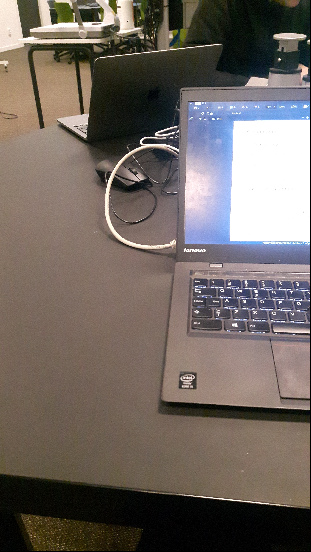
\includegraphics[scale=0.6]{./flow_src_0.jpg}
		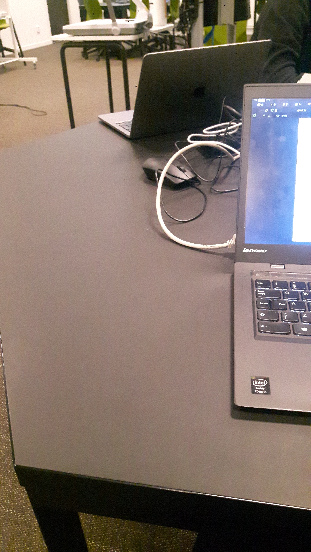
\includegraphics[scale=0.6]{./flow_src_1.jpg}
		\caption{The source images, in which one of the pictures some objects have been moved slightly more to the right}
	\end{center}
\end{figure}

\begin{figure}
	\begin{center}
		\begin{lstlisting}[language=Python]
#!/usr/bin/env python
import cv2
import numpy as np

feature_params = dict(
    maxCorners = 100,
    qualityLevel = 0.3,
    minDistance = 7,
    blockSize = 7,
)

lk_params = dict(
    winSize  = (15,15),
    maxLevel = 2,
    criteria = (cv2.TERM_CRITERIA_EPS | cv2.TERM_CRITERIA_COUNT, 10, 0.03)
)

old_frame = cv2.imread("./flow_src_0.jpg")
frame = cv2.imread("./flow_src_1.jpg")
old_gray = cv2.cvtColor(old_frame, cv2.COLOR_BGR2GRAY)
frame_gray = cv2.cvtColor(frame, cv2.COLOR_BGR2GRAY)

mask = np.zeros_like(old_frame)
p0 = cv2.goodFeaturesToTrack(old_gray, mask = None, **feature_params)
p1, st, err = cv2.calcOpticalFlowPyrLK(old_gray, frame_gray, p0, 
	None, **lk_params)

good_new = p1[st==1]
good_old = p0[st==1]
color = [255, 0, 0]

# go through all points of interest and mark them
for i,(new,old) in enumerate(zip(good_new,good_old)):
    a,b = np.array(np.round(new.ravel()), dtype=int)
    c,d = np.array(np.round(old.ravel()), dtype=int)
    mask = cv2.line(mask, (a,b),(c,d), color, 2)
    frame = cv2.circle(frame,(a,b),5, color,-1)
img = cv2.add(frame, mask)
cv2.imwrite("./flow_out.png", img)
		\end{lstlisting}
		\caption{Code using OpenCV's function for calculating optical flow}
	\end{center}
\end{figure}

\begin{figure}
	\begin{center}
		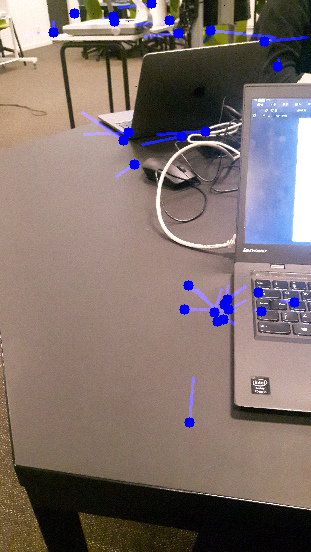
\includegraphics[scale=0.6]{./flow_out.png}
		\caption{Resulting image displaying how feature points have been moved from one image to the other}
	\end{center}
\end{figure}

	\subsubsection*{Write the function that is minimized in K-means. What are
the assumptions on the distributions of the points?
Given the points in the figure below, and the seeds to 2 centres in
(1;1.5) and (3;1). Compute two iterations of the k-means algorithm.}

\begin{figure}[H]
	\begin{center}
		\begin{lstlisting}[language=Python]
#!/usr/bin/env python
import math
import matplotlib.pyplot as plt

def k_means(seeds, points, distance_fn):
    results = [[] for _ in range(len(seeds))]
    for point in points:
        min_dist = math.inf
        min_element = 0
        for i in range(len(seeds)):
            new_dist = distance_fn(seeds[i], point)
            if new_dist < min_dist:
                min_dist = new_dist
                min_element = i
        (results[min_element]).append(point)
    new_seeds = seeds[:] # make sure that this is a copy
    for i in range(len(seeds)):
        cluster = results[i]
        if len(cluster) < 1:
            continue
        center = seeds[i]
        distance_sum = (0, 0)
        for point in cluster:
            dist = (center[0] - point[0], center[1] - point[1])
            distance_sum = (distance_sum[0] + dist[0], 
				distance_sum[1] + dist[1])
        mean = (distance_sum[0] / len(cluster), 
			distance_sum[1] / len(cluster))
        new_seeds[i] = (new_seeds[i][0] - mean[0], 
			new_seeds[i][1] - mean[1])
    return results, new_seeds
		\end{lstlisting}
		\caption{First half of the kmeans implementation}
	\end{center}
\end{figure}

\begin{figure}[H]
	\begin{center}
		\begin{lstlisting}[language=Python]
def distance(p1, p2):
    return math.sqrt((p2[0] - p1[0]) ** 2 + (p2[1] - p1[1]) ** 2)

def distance2(p1, p2):
    return (p2[0] - p1[0]) ** 2 + (p2[1] - p1[1]) ** 2

def plot_result(result, seeds):
    x_list = [list()] * len(result)
    y_list = [list()] * len(result)

    for i in range(len(x_list)):
        x_list[i] = [p[0] for p in result[i]]
        y_list[i] = [p[1] for p in result[i]]

    for i in range(len(x_list)):
        plt.plot(x_list[i], y_list[i], 'o')

    for seed in seeds:
        plt.plot(seed[0], seed[1], 'o')

    plt.xlim((-1, 6))
    plt.ylim((0, 3))
    plt.show()
        

seeds = [(1, 1.5), (3, 1)]
points = [
    (0, 0.8), (0, 0.5), (1.2, 0.4), (1.5, 0.8), (1, 1), (1.5, 1), 
    (2.5, 1), (3, 1), (3, 2), (4, 1.5), (4, 2.5), (5, 2)
]

regular_result, new_seeds = k_means(seeds, points, distance)
plot_result(regular_result, seeds)

regular_result, _ = k_means(new_seeds, points, distance)
plot_result(regular_result, new_seeds)
		\end{lstlisting}
		\caption{Second half of the kmeans implementation}
	\end{center}
\end{figure}

For this algorithm, I also gave a shot at comparing two distance methods. The first one is the standard euclidian distance function, whereas the second is the squared euclidian distance function. From my understanding, calculating the square root of a number is a (when compared to other various arithmetic operations) rather slow calculation to perform performance-wise. Seeing as we are only comparing the results of the distance function, it does not matter if the result is squared or not, as long as the calculated distance are to scale with each other. This being a python implementation and the dataset being comparatively small means that the code is just about as performant regardless of the distance function used, but it is still some food for thought. 

\begin{figure}[H]
	\begin{center}
		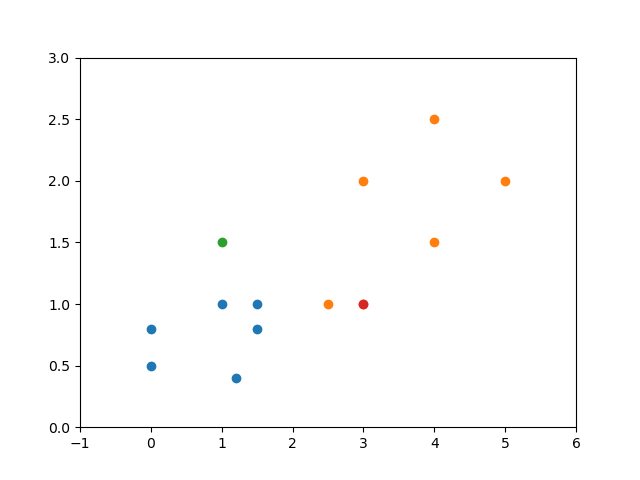
\includegraphics[scale=0.5]{./kmeans_iter_1.png}
		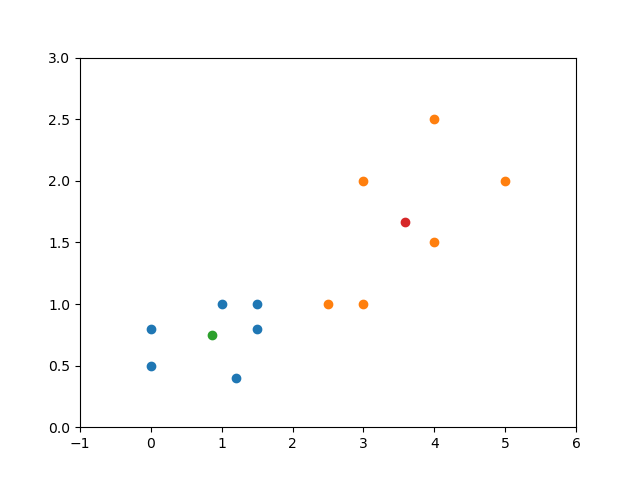
\includegraphics[scale=0.5]{./kmeans_iter_2.png}
		\caption{The results of the first two iterations of the kmeans algorithm on the given dataset. Blue and orange points represent the different classes, whereas the green and the red points represent the ''centers'' of the blue and orange classes, respectively.}
	\end{center}
\end{figure}

	\subsubsection*{Implement a segmentation algorithm for colour images.Choose between a mean-shift algorithm (Ex. 5.5 in the book) or a
k-means algorithm.}

\begin{figure}[H]
	\begin{center}
		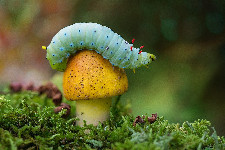
\includegraphics[scale=0.8]{./caterpillar.jpg}
		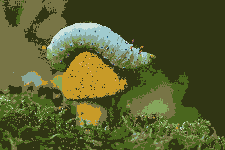
\includegraphics[scale=0.8]{./kmeans_segmentation.png}
		\caption{A before-after comparison of the kmeans-segmentation algorithm that was implemented.}
	\end{center}
\end{figure}

\begin{figure}[H]
	\begin{center}
		\begin{lstlisting}[language=Python]
#!/usr/bin/env python
import math
import random
import cv2
import numpy as np

def distance(a, b):
    return int(a[0] - int(b[0])) ** 2 +int(a[1] - int(b[1])) ** 2 
		+ int(a[2] - int(b[2])) **2

def kmeans_seeds(k):
    centers = [[] for _ in range(k)]
    for i in range(k):
        centers[i] = [random.randint(0, 255), random.randint(0, 255), 
			random.randint(0, 255)]
    return centers
		\end{lstlisting}
		\caption{Some helper functions for implementing the kmeans-algorithm}
	\end{center}
\end{figure}

\begin{figure}[H]
	\begin{center}
		\begin{lstlisting}[language=Python]
def kmeans(original_data, data, centers):
    new_image = np.copy(data)
    new_centers = np.copy(centers)
    clusters = np.zeros(data.shape[:2])
    for i in range(len(data)):
        for j in range(len(data[i])):
            distances = [distance(data[i][j], center) for center in centers]
            min_distance = math.inf
            min_index = 0

            for k in range(len(distances)):
                if distances[k] < min_distance:
                    min_distance = distances[k]
                    min_index = k

            new_image[i][j] = centers[min_index]
            clusters[i][j] = min_index
    for k in range(len(new_centers)):
        r, g, b, n = 0, 0, 0, 0
        g = 0
        b = 0
        n = 0
        for i in range(len(clusters)):
            for j in range(len(clusters[i])):
                cluster = clusters[i][j]
                if cluster == k:
                    r += original_data[i][j][0]
                    g += original_data[i][j][1]
                    b += original_data[i][j][2]
                    n += 1
        if n == 0:
            continue

        r /= n
        g /= n
        b /= n

        new_centers[k][0] = r
        new_centers[k][1] = g
        new_centers[k][2] = b

    return new_image, new_centers
		\end{lstlisting}
		\caption{The actual implementation of the kmeans segmentation algorithm}
	\end{center}
\end{figure}

\begin{figure}[H]
	\begin{center}
		\begin{lstlisting}[language=Python]
path = "./caterpillar.jpg"
img = cv2.imread(path)

original_data = img

centers = kmeans_seeds(20)
for _ in range(8):
	img, centers = kmeans(original_data, img, centers)
	cv2.imwrite("kmeans_out.png", img)
		\end{lstlisting}
		\caption{Lastly, the actual usage of the segmentation algorithm}
	\end{center}
\end{figure}

For this assignment, I chose to use random color values as the seeds. This impacted the result of the algorithm greatly, as the first iterations of the algorithm resulted in a wild array of colors, depending on the seeds generated. Over time, the generated image began to look more and more like the original image, as the seed values converged into something more appropriate for the picture.

\section*{Assignment 6}
	\subsubsection*{Identify and download an implementation of structure from motion, which also shares the source code. In the source code, point out the main processing steps of structure from motion.}

	I am a bit unsure as to if my understanding regarding what the code I have selected to present actually \emph{actually} does, but it seems to align with what Mårten discussed during the lecture.

	Inside my framework, I found a function named \lstinline{compute_depthmap}, which sounds awfully central to the type of work necessary for this problem. It mentions ''neighbours'' and ''patches'' a couple of times within the code, which reminded me about how Mårten discussed the feature detection of each individual source image, to later find corresponding feature points between these source which, ultimately, is then used to understand how the different images relate to each other.

	\begin{figure}[H]
		\begin{center}
			\begin{lstlisting}[language=Python]
def compute_depthmap(arguments):
    """Compute depthmap for a single shot."""
    log.setup()

	# During the arg unpack, neighbors are present, suggesting that
	# several images may be present during the course of the algorithm
    data: UndistortedDataSet = arguments[0]
    neighbors = arguments[1]
    min_depth = arguments[2]
    max_depth = arguments[3]
    shot = arguments[4]

    method = data.config["depthmap_method"]

    if data.raw_depthmap_exists(shot.id):
        logger.info("Using precomputed raw depthmap {}".format(shot.id))
        return
    logger.info("Computing depthmap for image {0} with {1}".format(shot.id, method))

	# Class for estimating depth
    de = pydense.DepthmapEstimator()
    de.set_depth_range(min_depth, max_depth, 100)
    de.set_patchmatch_iterations(data.config["depthmap_patchmatch_iterations"])
    de.set_patch_size(data.config["depthmap_patch_size"])
    de.set_min_patch_sd(data.config["depthmap_min_patch_sd"])
    add_views_to_depth_estimator(data, neighbors, de)
	# Supposedly some sort of method selection, certain methods
	# seem to suggest operating on different patches, meaning
	# they might try to find common occurences in different images
    if method == "BRUTE_FORCE":
        depth, plane, score, nghbr = de.compute_brute_force()
    elif method == "PATCH_MATCH":
        depth, plane, score, nghbr = de.compute_patch_match()
    elif method == "PATCH_MATCH_SAMPLE":
        depth, plane, score, nghbr = de.compute_patch_match_sample()
    else:
        raise ValueError(
            "Unknown depthmap method type "
            "(must be BRUTE_FORCE, PATCH_MATCH or PATCH_MATCH_SAMPLE)"
        )
    good_score = score > data.config["depthmap_min_correlation_score"]
    depth = depth * (depth < max_depth) * good_score
    # Save and display results
    neighbor_ids = [i.id for i in neighbors[1:]]
    data.save_raw_depthmap(shot.id, depth, plane, score, nghbr, neighbor_ids)
			\end{lstlisting}
			\caption{Excerpt of the OpenSFM framework (dense.py).}
		\end{center}
	\end{figure}

	\subsubsection*{Take a number of pictures of (or film) a scene with an objects in it. Carry out structure from motion by using the implementation you have downloaded.}

	I dotted down a couple of images from a test dataset contained within the implementation, presenting me with these results:

\begin{figure}[H]
	\begin{center}
		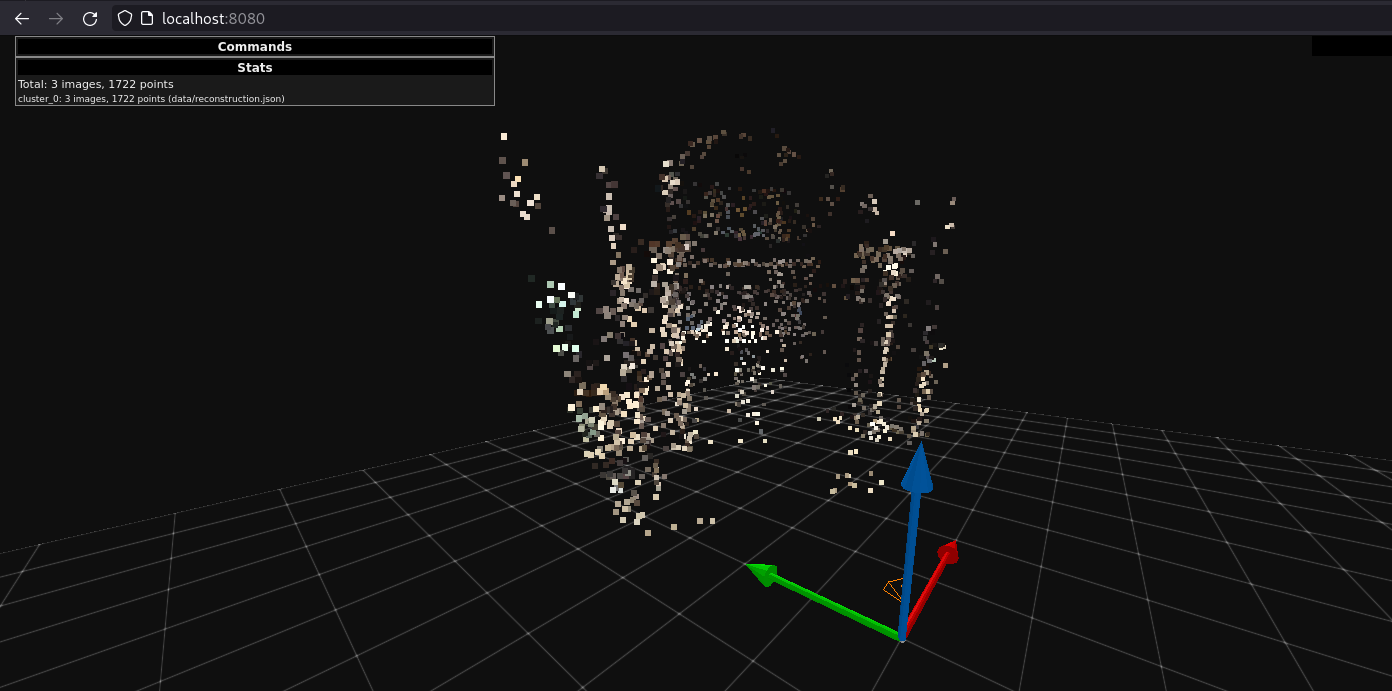
\includegraphics[scale=0.4]{./sfm_webview.png}
		\caption{The resulting ''model'' created from running the software on one of the provided datasets and serving it to the browser.}
	\end{center}
\end{figure}

\begin{figure}[H]
	\begin{center}
		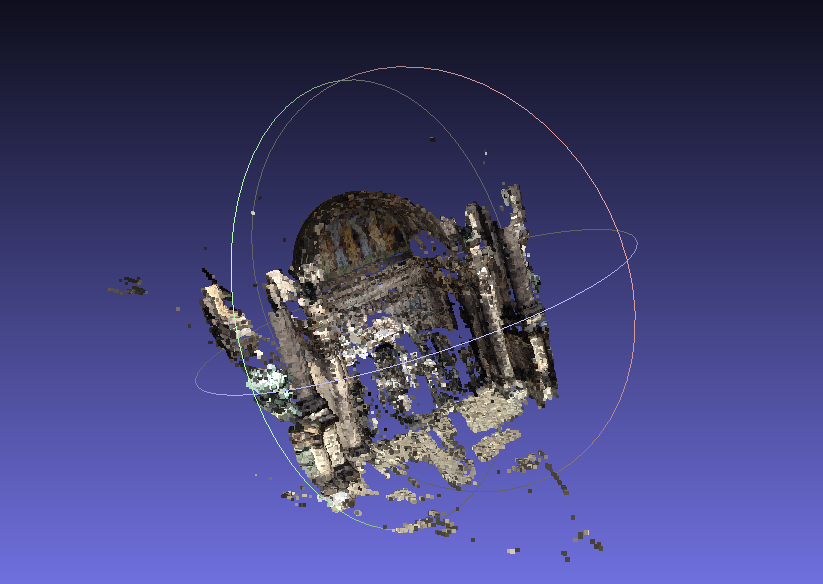
\includegraphics[scale=0.5]{./sfm_meshlab.png}
		\caption{The resulting point cloud presented using Meshlab created by running the software in dense mode, which produces an observably denser model of the recreated structure.}
	\end{center}
\end{figure}

\begin{figure}[H]
	\begin{center}
		\includegraphics*[scale=0.4]{./sfm_blender.png}
		\caption{The same point cloud as the one above, but presented in Blender.}
	\end{center}
\end{figure}

\section*{Assignment 7}
	\subsubsection*{Define an arbitrary triangle with three vertices of your choosing. Select two points, one within and one outside the triangle. Use the above equations to validate that you can determine if each point is covered by the triangle or not.}
	\begin{figure}
		\begin{center}
			\begin{lstlisting}[language=Python]
#!/usr/bin/env python
import matplotlib.pyplot as plt

def sub(a, b):
    return (a[0] - b[0], a[1] - b[1])

def dot(a, b):
    return a[0] * b[0] + a[1] * b[1]

def is_inside(p0, p1, p2, pt):
    t = sub(p1, p0)
    n = (t[1], -t[0])
    inside_check_0 = dot(sub(pt, p0), n) < 0

    t = sub(p2, p1)
    n = (t[1], -t[0])
    inside_check_1 = dot(sub(pt, p1), n) < 0

    t = sub(p0, p2)
    n = (t[1], -t[0])
    inside_check_2 = dot(sub(pt, p2), n) < 0

    return inside_check_0 and inside_check_1 and inside_check_2

p = [	# triangle points
    (-0.5, 0),
    ( 0.5, 0),
    ( 0,   1),
]

should_be_inside = [(0, 0.5), (0, 0.2), (0.3, 0.1)]
should_be_outside = [(1, -0.5), (0.5, 0.5), (0, -0.5)]

for inside in should_be_inside:
    inside_plot_data = 'go' if is_inside(p[0], p[1], p[2], inside) else 'ro'
    plt.plot([inside[0]], [inside[1]], inside_plot_data)
plt.plot([p[0][0], p[1][0]], [p[0][1], p[1][1]], 'b')
plt.plot([p[1][0], p[2][0]], [p[1][1], p[2][1]], 'b')
plt.plot([p[2][0], p[0][0]], [p[2][1], p[0][1]], 'b')
plt.show()

for outside in should_be_outside:
    outside_plot_data = 'go' if is_inside(p[0], p[1], p[2], outside) else 'ro'
    plt.plot([outside[0]], [outside[1]], outside_plot_data)
plt.plot([p[0][0], p[1][0]], [p[0][1], p[1][1]], 'b')
plt.plot([p[1][0], p[2][0]], [p[1][1], p[2][1]], 'b')
plt.plot([p[2][0], p[0][0]], [p[2][1], p[0][1]], 'b')
plt.show()
			\end{lstlisting}
		\end{center}
	\end{figure}

	The primary resource that was used to finish this exercise was the slides from lecture 7, in particular those titled \textit{''Point within triangle''} and \textit{''Pixel within triangle''}. The forumula used to calculate the normal to a line and the ray of this normal was repeated for each line being a part of the triangle, with the results plotted using matplotlib.

	\begin{figure}
		\begin{center}
			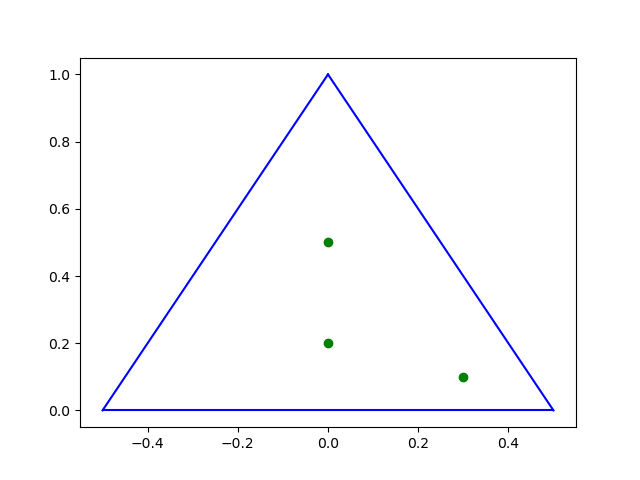
\includegraphics[scale=0.4]{./inside_triangle.png}
			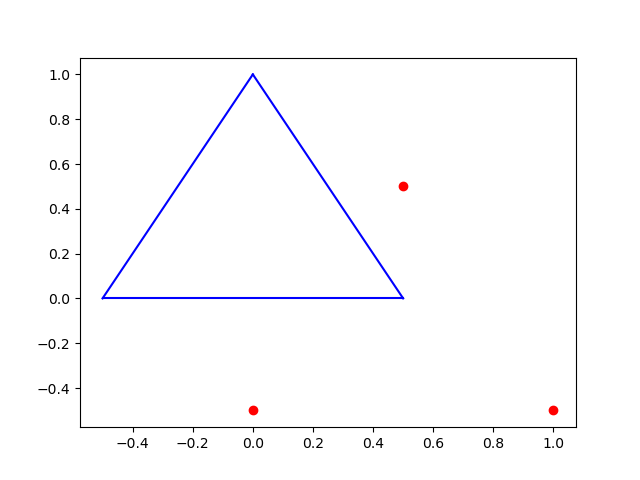
\includegraphics[scale=0.4]{./outside_triangle.png}
			\caption{Figure displaying two plots who describe the results of the function, green dots are considered to be inside the triangle, whereas red dots are considered to be outside the triangle.}
		\end{center}
	\end{figure}

	\subsubsection*{Evaluate the Phong shading model and plot how the specular light change as a function of angle $\phi$ between viewing and reflection vector, as well as specularity constant $\alpha$. Select appropriate figures for showing these variations.}

	\begin{figure}[H]
		\begin{center}
			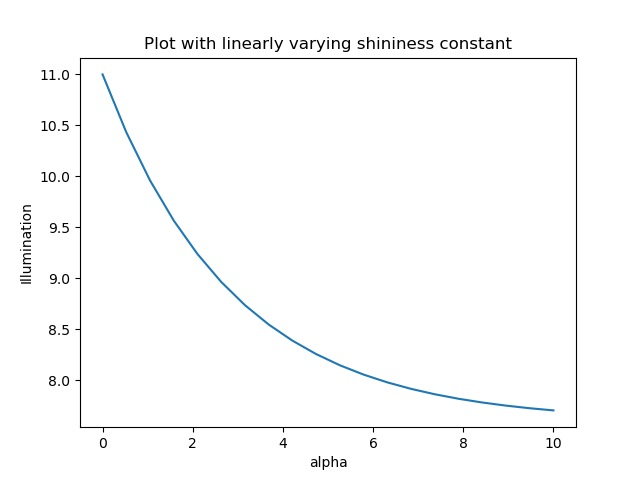
\includegraphics[scale=0.4]{./alpha_plot.png}
			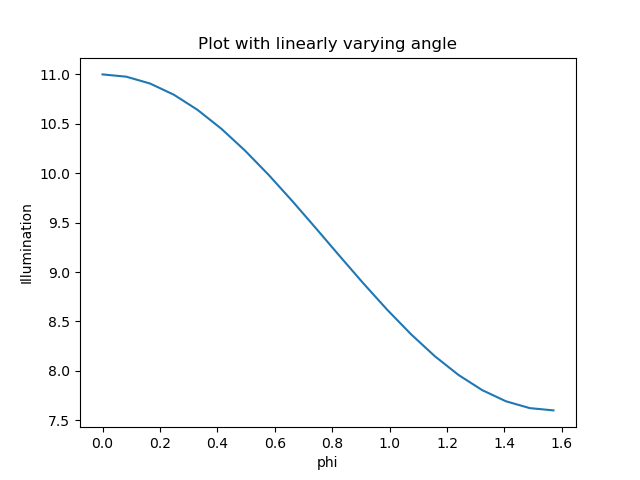
\includegraphics[scale=0.4]{./phi_plot.png}
			\caption{Figure displaying the change in illumination when varying either the $\alpha$ or $\phi$ value within the phong illumination model.}
		\end{center}
	\end{figure}

	As can be seen in the figure above, the illumination of an object is at its brightest when the source of light is directly above the object, e.g when the angle ($\phi$) between the light source and the object normal is 0. Likewise, increasing the shininess constant will have a diminishing effect on reducing the illumination depending on how high you set the shininess constant.

	\begin{figure}[H]
		\begin{center}
			\begin{lstlisting}[language=Python]
#!/usr/bin/env python
import numpy as np
import matplotlib.pyplot as plt

"""
I = k_a * i_a + k_d * i_d + k_s(cos(phi))^a i_l

i_a = ambient light
i_d = diffuse light
i_s = specular light
a = shininess constant
"""
def phong(k_a, k_d, k_s, i_a, i_d, i_l, a, phi):
    return k_a * i_a + k_d * i_d + k_s * (np.cos(phi) ** a) * i_l

i_a = 2.5
i_d = 1.3
i_l = 1.7

k_a = 2.0
k_d = 2.0
k_s = 2.0

a = np.linspace(0.0, 10.0, num=20)
phi = np.linspace(0.0, np.pi / 2, num=20)

y0 = [phong(k_a, k_d, k_s, i_a, i_d, i_l, x, np.pi / 4.) for x in a]
y1 = [phong(k_a, k_d, k_s, i_a, i_d, i_l, 2.0, x) for x in phi]

ax = plt.axes()
plt.plot(a, y0)
plt.title("Plot with linearly varying shininess constant")
ax.set_xlabel("alpha")
ax.set_ylabel("Illumination")
plt.show()
ax = plt.axes()
plt.plot(phi, y1)
plt.title("Plot with linearly varying angle")
ax.set_xlabel("phi")
ax.set_ylabel("Illumination")
plt.show()
			\end{lstlisting}
		\end{center}
	\end{figure}

	\subsubsection*{Use python, the pyglet package, and the ratcave package to create a 3D image of a 3D-model (download or use any of the basic primitives). As as much functionality to our application as you want, but basic Lambertian shading and ambient light is a requirement.}

	\begin{figure}[H]
		\begin{center}
			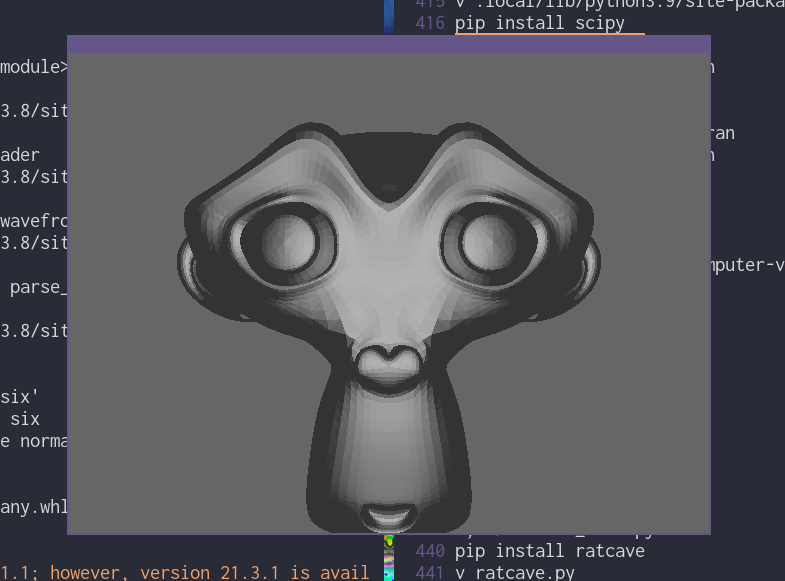
\includegraphics[scale=0.4]{./monkey_man.png}
			\caption{A basic 3D-model rendered using ambient lights and lambertian shading.}
		\end{center}
	\end{figure}

	\begin{figure}[H]
		\begin{center}
			\begin{lstlisting}[language=Python]
 #!/usr/bin/env python3.8
import pyglet
import ratcave as rc
from pyglet.window import key

x = 0

vert_shader = """
#version 120

attribute vec3 vertexPosition;
attribute vec3 normalPosition;
uniform mat4 model_matrix, normal_matrix;
uniform mat4 view_matrix = mat4(1.0);
uniform mat4 projection_matrix = mat4(
    vec4(1.38564062,  0.,  0.,  0.),
    vec4(0.,  1.73205078,  0.,  0.),
    vec4(0., 0., -1.01680672, -1. ),
    vec4(0., 0., -0.20168068, 0.)
);

varying vec4 vVertex;
varying vec3 normal;

void main()
{
    gl_Position = projection_matrix * view_matrix 
		* model_matrix * vec4(vertexPosition, 1.0);
    vVertex = model_matrix * vec4(vertexPosition, 1.0);
    normal = normalize(normal_matrix * vec4(normalPosition, 1.0)).xyz;
}
"""
			\end{lstlisting}
			\caption{The vertex shader used in the script, heavily influenced by the phong shader code presented on the ratcave github page.}
		\end{center}
	\end{figure}

	\begin{figure}[H]
		\begin{center}
			\begin{lstlisting}[language=Python]
frag_shader = """
#version 120
uniform vec3 camera_position, light_position;
uniform vec3 diffuse, ambient;

varying vec3 normal;
varying vec4 vVertex;

vec4 doLambert(vec3 vertex, vec3 normal, vec3 light_position, 
		vec3 camera_position, vec3 ambient, vec3 diffuse) {
    vec4 color = vec4(ambient, 1.);
    vec3 light_direction = normalize(light_position - vertex);

    vec3 reflectionVector = reflect(light_direction, normalize(normal));
    float cosAngle = max(0.0, -dot(normalize(camera_position - vertex),
			reflectionVector));
	
	// hijacking one of the example shaders present in the
	// ratcave github :)

	// set ambient light
    ambient = vec3(0.2, 0.2, 0.2);
	// set lamberitan light
    vec3 i = ambient + (cosAngle * vec3(0.5, 0.5, 0.5));

    return vec4(i, 1);
}

void main()
{
    gl_FragColor = doLambert(vVertex.xyz, normal, light_position, 
		camera_position, ambient, diffuse);

}
"""
			\end{lstlisting}
			\caption{The fragment shader used in the script, heavily influenced by the phong shader code presented on the ratcave github page, with some tweaks made to convert it into a lambertian shading model.}
		\end{center}
	\end{figure}
	\begin{figure}[H]
		\begin{center}
			\begin{lstlisting}[language=Python]

shader = rc.Shader(vert=vert_shader, frag=frag_shader)

window = pyglet.window.Window()
pyglet.clock.schedule(lambda dt: dt)

file = rc.resources.obj_primitives
monkey = rc.WavefrontReader(file).get_mesh("Monkey")
monkey.position.xyz = 0, 0, -2

scene = rc.Scene(meshes=[monkey])

# minor tweaks, can move the scene around
@window.event
def on_key_press(symbol, _):
    global x
    if symbol == key.RIGHT:
       x += 0.05
    elif symbol == key.LEFT:
       x -= 0.05
    scene.camera.position.xyz = x, 0, 0

@window.event
def on_draw():
    with shader:
        scene.draw()

pyglet.app.run()
			\end{lstlisting}
			\caption{Main components of the rendering script: some callbacks to when rendering and keyboard actions should be accounted for as well as the loading of a mesh and a shader.}
		\end{center}
	\end{figure}

	\newpage
	\printbibliography
\end{document}
